\section{Introduction}

In traditional video game search engines, the query pertains to titles and genres. If the user does not know the name of the game they are looking for, this can lead to frustration. Our search engine allows the user to specify which section of the game's description they want to search over. For example, the user could choose to search over summaries if they know the general characteristics of the game they desire.

\section{Collecting the data}
The data used in our database came from scraping wikipedia articles for video games. Wikipeida offers large lists of games for each major console. The scraper was designed to pull information from the info box, description, and main body of each page.



The infobox (Figure \ref{fig:infobox}) contains most of the game's information we will collect

\begin{figure}[h!]

\includegraphics[width=1in]{infobox}
\caption{Wikipedia Infobox}
\label{fig:infobox}
\end{figure}

There were 16,508 games collected in total. This data was collected into a JSON format (Figure \ref{fig:JSONsample}) so that the indexer program could easily add the data into the Whoosh! index. 

\begin{minipage}[H]{0.4\textwidth}
\begin{verbatim}
{
  "title": "007 Racing",                
  "url": "https://en.wikipedia.org/...",
  "image": "https://upload.wikimedi...",
  "release": " November 2000",          
  "developer": "Eutechnyx",             
  "publisher": "EA Games",              
  "genres": "Racing",                   
  "modes": "Single-player, multiplayer",
  "platforms": "PlayStation",           
  "summary": "007 Racing is a 2000 ...",
  "body": "In 007 Racing the player..."
}
\end{verbatim}
\captionof{figure}{Sample tuple from collected data}
\label{fig:JSONsample}
\end{minipage}

\section{Indexing the data}
The Whoosh! python module was used to index the collected data. We chose to collect and save the url, title, image url, release date, developers, publishers, genres, game modes, platforms, and summary (Figure \ref{fig:whooshschema}). These will be potential data points that could be returned to the user. The body text we collected will not need to be returned to the user so it was indexed but not stored. Choosing not to store the body text saved nearly 70MB of space from our index. Whoosh will work together with other modules in order to serve the data from the backend api to the frontend.

\begin{figure}[h]
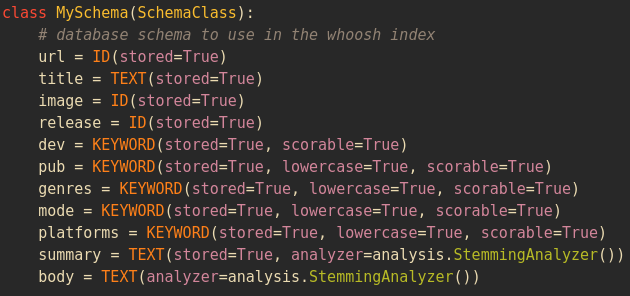
\includegraphics[width=3in]{whooshSchema}
\caption{Whoosh Schema}
\label{fig:whooshschema}
\end{figure}

\section{Serving the data}
We are using the Flask module as an API to connect the backend to the frontend. The React frontend app will be able to request data through the API in order to display what the user wants.

\section{Viewing the data}
The data will be displayed to the user using the React JavaScript library. React was chosen due to its high customizability and open source foundation. 

\subsection{Design Choices}
A simple background, logo, and buttons were chosen to create a sleek home page. The search bar was created longer to fit six words, because the query will also search through the descriptions of the games. This allows the user to still find the game if he cannot remember the exact title. 

In the search results page, the background is the same as the home page to create a continuous feel throughout the web app. The results are displayed in a grid 2 results wide and 5 results tall to fit 10 results per page. 

\subsection{Functionality}
Each separate page and component (search bar, tuple) displayed to the user is created in a separate javascript file. The users queries and search options are easily recorded and handled using state variables. These state variables make handling user requests easy, because as the state variable is updated the components shown to the user can be updated. 

The color, fonts, and format are assigned in CSS files. Each page has a separate CSS file. 

\subsection{Citations}
Citations to articles

\section{Conclusions}
This paragraph will end the body of this sample document.
Remember that you might still have Acknowledgments or
Appendices; brief samples of these
follow.  There is still the Bibliography to deal with; and
we will make a disclaimer about that here: with the exception
of the reference to the \LaTeX\ book, the citations in
this paper are to articles which have nothing to
do with the present subject and are used as
examples only.
\end{document}  % This is where a 'short' article might terminate



%\appendix
%Appendix A
%\subsection{Introduction}
%\subsection{Collecting the data}
%\subsection{Indexing the data}
%\subsection{Serving the data}
%\subsection{Viewing the data}
%\subsection{Citations}
%\subsection{Conclusions}
%\subsection{References}